\documentclass{beamer}
\usetheme{Madrid}
\usecolortheme{seahorse}
\title{FGC Evening Service}
\subtitle{Weekday evening, 20:00--24:00}
\author{Prepared for the transport authority}
\date{}
\begin{document}
\frame{\titlepage}
\begin{frame}{Evening service is uneven}
Riders on the thinner-served lines wait far longer for a train than riders on the core network.

\end{frame}
\begin{frame}{The gap is large}
The best line runs every 6 minutes; the worst waits 240 minutes between trains - 40 times longer.
\[ \frac{240}{6} = 40\times \]
\begin{center}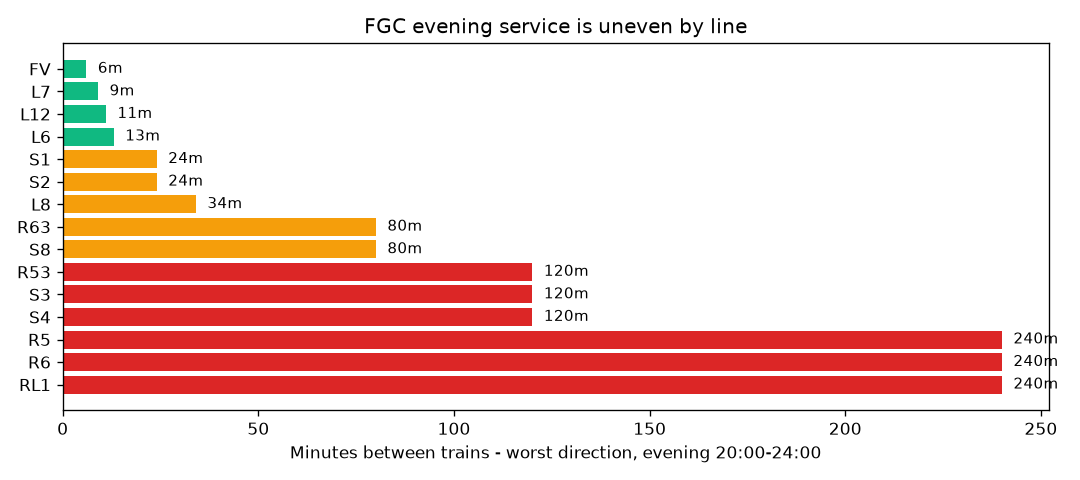
\includegraphics[width=0.62\textwidth]{fgc-evening-frequency.png}\end{center}
\end{frame}
\begin{frame}{Six lines are barely served}
R53, S3, S4, R5, R6 and RL1 wait two hours or more between evening trains.

\end{frame}
\begin{frame}{The imbalance is structural}
The best line runs 20 trains an hour; the worst runs one every two hours.

\end{frame}
\begin{frame}{Recommendation}
Add evening trips on the lines waiting two hours or more, then re-check after the next timetable change.

\end{frame}
\end{document}
